% \documentclass[aspectratio=169,notes]{beamer}
\documentclass[aspectratio=169]{beamer}
\usetheme[faculty=phil]{fibeamer}
\usepackage{polyglossia}
\setmainlanguage{english} %% main locale instead of `english`, you
%% can typeset the presentation in either Czech or Slovak,
%% respectively.
\setotherlanguages{russian} %% The additional keys allow
%%
%%   \begin{otherlanguage}{czech}   ... \end{otherlanguage}
%%   \begin{otherlanguage}{slovak}  ... \end{otherlanguage}
%%
%% These macros specify information about the presentation
\title[AGLA1]{Analytical Geometry and Linear Algebra I, Lab 6} %% that will be typeset on the
\subtitle{Line in plane \\ \  \\ \    
         } %% title page.
\author{Oleg Bulichev}
%% These additional packages are used within the document:
\usepackage{ragged2e}  % `\justifying` text
\usepackage{booktabs}  % Tables
\usepackage{tabularx}
\usepackage{tikz}      % Diagrams
\usetikzlibrary{calc, shapes, backgrounds}
\usepackage{amsmath, amssymb}
\usepackage{url}       % `\url`s
\usepackage{listings}  % Code listings
% \usepackage{subfigure}
\usepackage{floatrow}
\usepackage{subcaption}
\usepackage{mathtools}
\usepackage{todonotes}
\usepackage{fontspec}
\usepackage{multicol}
\usepackage{pdfpages}
\usepackage{wrapfig}
\usepackage{animate}
\usepackage{booktabs}
\usepackage{multirow}

\graphicspath{{resources/}}
\frenchspacing

\setbeamertemplate{caption}[numbered]
\usetikzlibrary{graphs}

% \usepackage[backend=biber,style=ieee,autocite=footnote]{biblatex}
% \addbibresource{biblio.bib}
% \DefineBibliographyStrings{english}{%
%   bibliography = {References},}

\newcommand{\oleg}[2][] {\todo[color=red, #1] {OLEG:\\ #2}}
\newcommand{\fbckg}[1]{\usebackgroundtemplate{\includegraphics[width=\paperwidth]{#1}}}%frame background

\usepackage[framemethod=TikZ]{mdframed}
\newcommand{\dbox}[1]{
\begin{mdframed}[roundcorner=3pt, backgroundcolor=yellow, linewidth=0]
\vspace{1mm}
{#1}
\vspace{1mm}
\end{mdframed}
}

\begin{document}
\setlength{\abovedisplayskip}{0pt}
\setlength{\belowdisplayskip}{0pt}
\setlength{\abovedisplayshortskip}{0pt}
\setlength{\belowdisplayshortskip}{0pt}

\fbckg{fibeamer/figs/title_page.png}
\frame[c]{\setcounter{framenumber}{0}
    \usebeamerfont{title}%
    \usebeamercolor[fg]{title}%
    \begin{minipage}[b][6.5\baselineskip][b]{\textwidth}%
        \textcolor{black}{\raggedright\inserttitle}
    \end{minipage}
    % \vskip-1.5\baselineskip

    \usebeamerfont{subtitle}%
    \usebeamercolor[fg]{framesubtitle}%
    \begin{minipage}[b][3\baselineskip][b]{\textwidth}
        \raggedright%
        \insertsubtitle%
    \end{minipage}
    \vskip.25\baselineskip
}
%   \frame[c]{\maketitle}
\note{
    \begin{enumerate}
        \item Чилл пара

    \end{enumerate}
}

\fbckg{fibeamer/figs/common.png}


\begin{frame}[c]{Questions from the class}
\framesubtitle{}
\centering
    \textit{ \Large No questions for today}
\end{frame}

\begin{frame}[t]{Objectives}
\framesubtitle{}
    \begin{itemize}
        \item To see the structure of all formulas, which were covered
        \item To understand how to transform one from to another and vise-versa 
        \item How to apply the knowledge
    \end{itemize}
\end{frame}

\begin{frame}[t]{Type of elements}
\framesubtitle{}
    \vspace{-0.6cm}
    \begin{figure}[H]
        \centering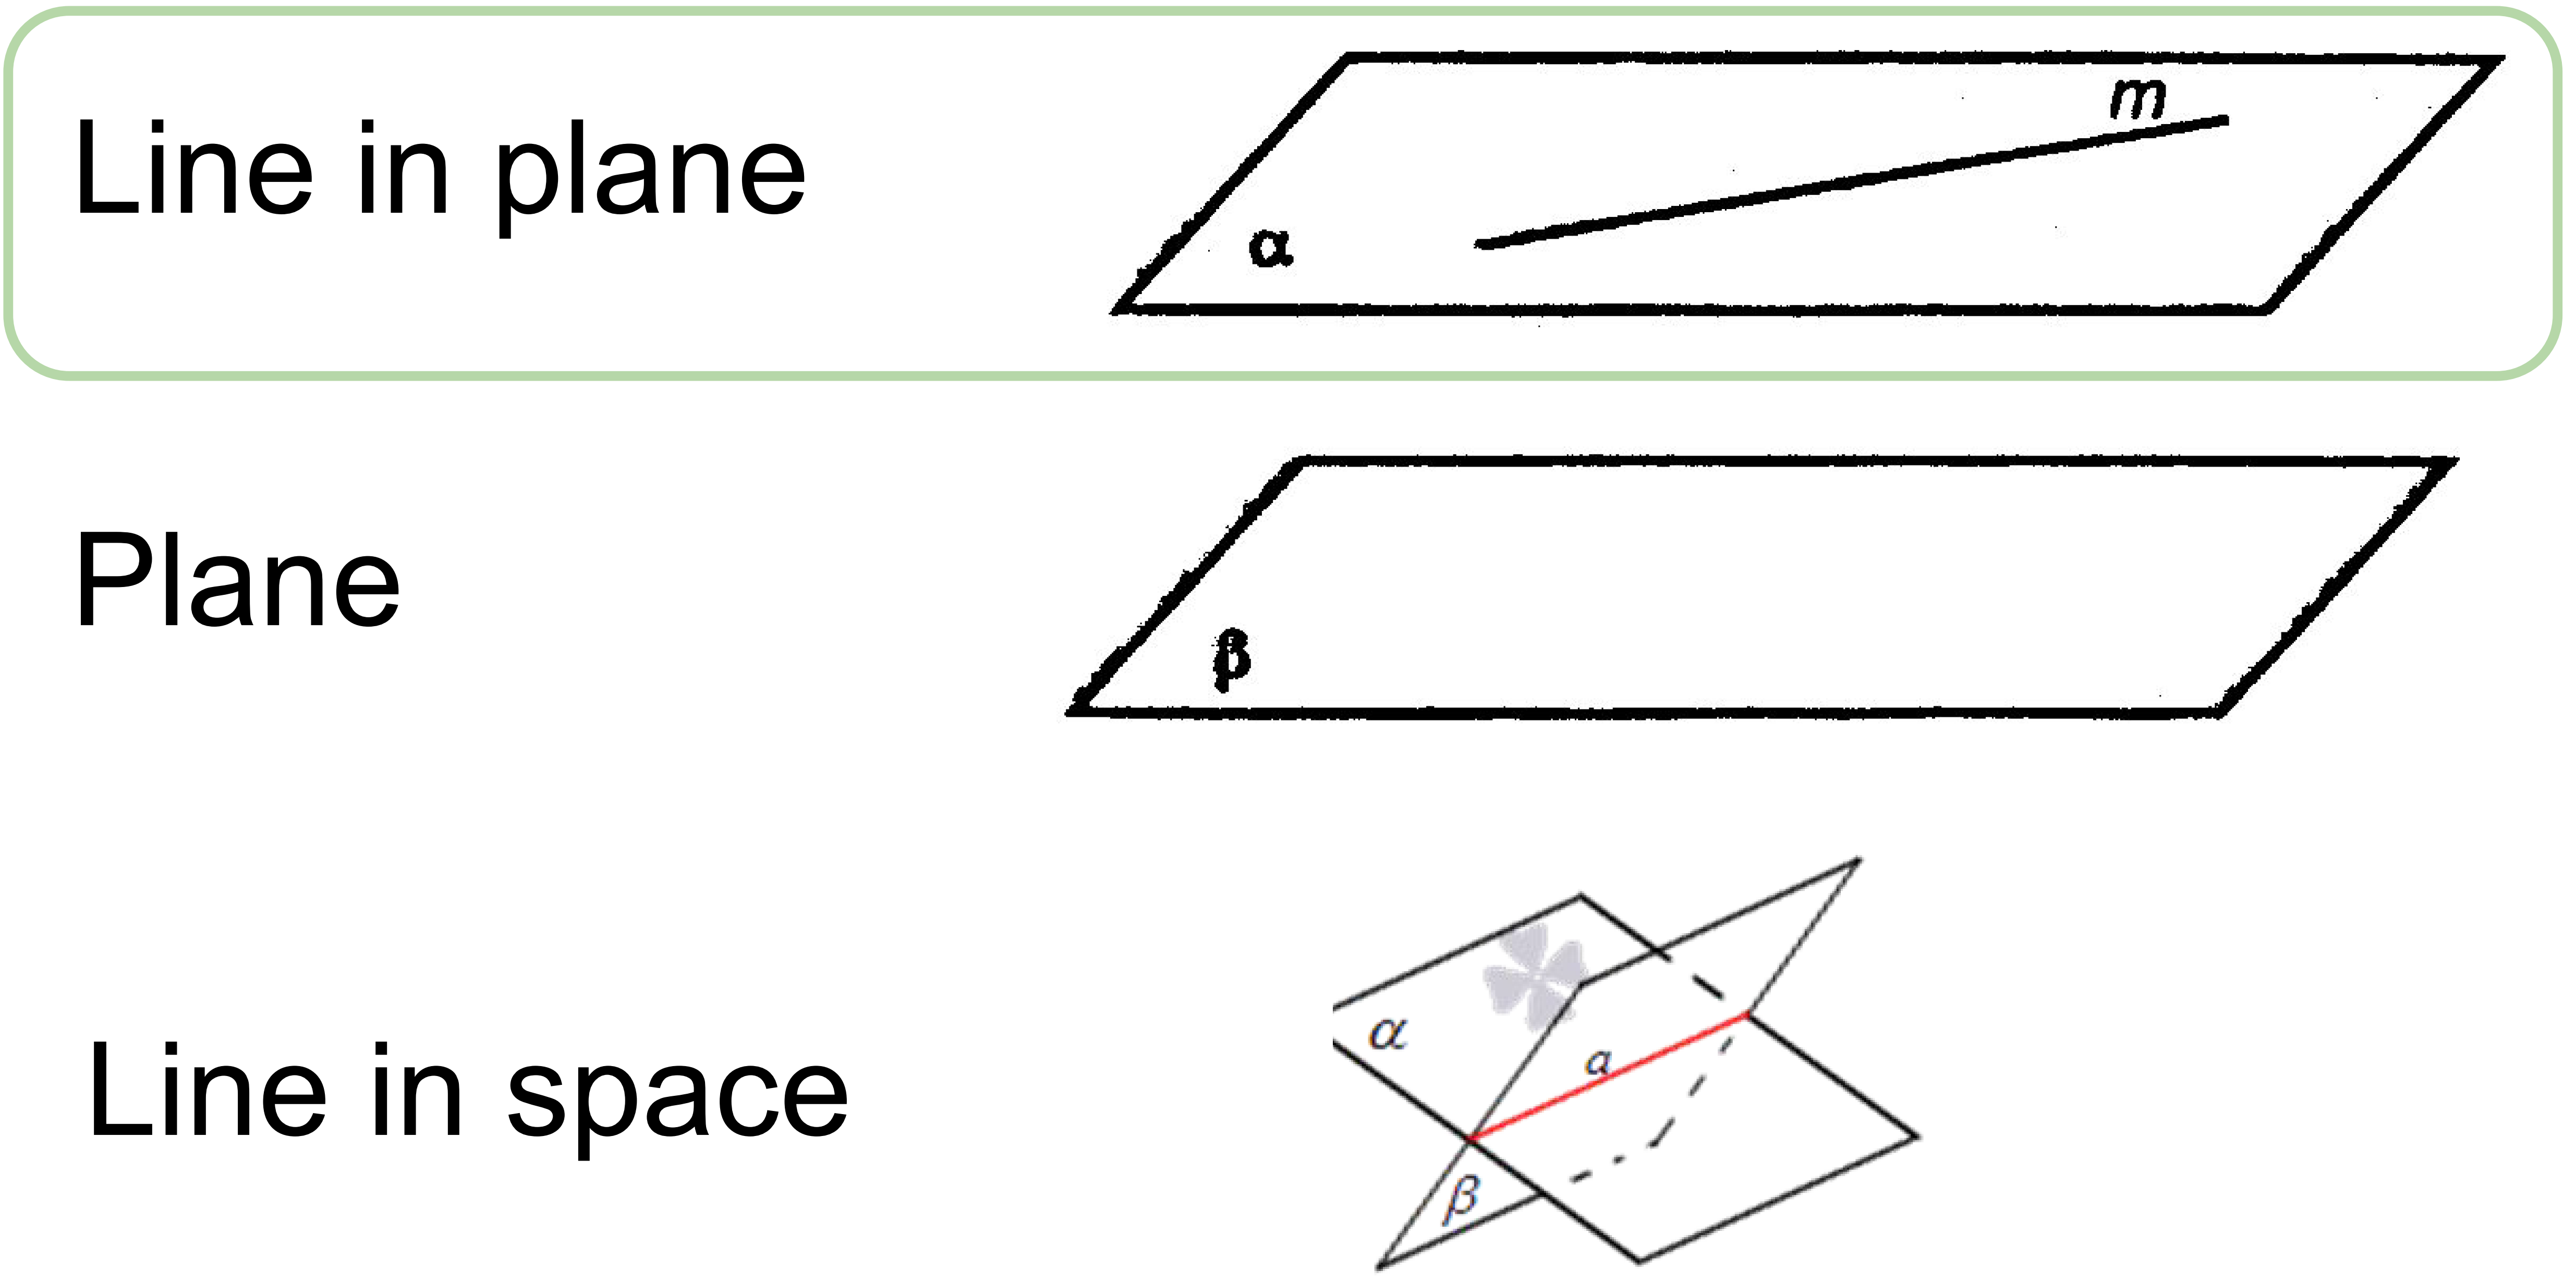
\includegraphics[height=6cm,width=1\textwidth,keepaspectratio]{line_in_plane.png}
        \label{fig:line_in_plane.png}
    \end{figure}
\end{frame}

\begin{frame}[t]{Computer Aided Design}
    \framesubtitle{Form types}
    \begin{table}[H]
        \centering
        \begin{tabular}{llll}
        \textbf{Type} & \textbf{Form} & \textbf{Example} & \textbf{Description} \\ 
        \hline
        \textit{Explicit} & $y=f(x)\,\!$ & $y=mx+b\,\!$ & Line \\
        \textit{Implicit} & $f(x,y)=0\,\!$ & $\left(x-a\right)^{2}+\left(y-b\right)^{2}=r^{2}$ & Circle \\
        \multirow{2}{*}{\textit{Parametric}} & \multirow{2}{*}{${\displaystyle x={\frac {g(t)}{w(t)}};\,\!} {\displaystyle y={\frac {h(t)}{w(t)}}}$} & $x=a_{0}+a_{1}t;\,\! {\displaystyle y=b_{0}+b_{1}t\,\!}$ & Line \\
         &  & $x=a+r\,\cos t;\,\! {\displaystyle y=b+r\,\sin t\,\!}$ & Circle
        \end{tabular}
        \end{table}
    \end{frame}

\begin{frame}[t]{Line in plane}
\framesubtitle{Formulas}
\scriptsize
\vspace{-0.4cm}
\begin{multicols}{2}
    \begin{enumerate}
        \item \textbf{\textit{General equation}} $Ax + By + C = 0$, where \\ $C = -Ax_0 - By_0$
        \item \textbf{\textit{Slope-intercept}} $y = kx + b$, where $k = tan(X\text{-axis} \hat{\ }y(x))$ -- slope
         \item \textbf{\textit{Passing through two points}} $\dfrac{x-x_1}{x_2-x_1} = \dfrac{y-y_1}{y_2-y_1}$; slope is $k = \dfrac{y_2-x_1}{x_2-x_1}$\\ where $x_{1,2}$, $y_{1,2}$ are some particular coordinates of points on the line
        \item \textbf{\textit{Canonical}} $\dfrac{x-x_0}{a_x} = \dfrac{y-y_0}{a_y}$,\\ where $x_0$, $y_0$ is a point on the line and $a_x$, $a_y$ -- direction vector coefficients on a basis
        \item \textbf{\textit{Parametric}} $\vec{r} = \vec{r_0} + \tau \vec{a}=\left\{\begin{matrix} x = x_0 + \tau a_x 
    \\ y = y_0 + \tau a_y 
    \end{matrix}\right.$, where $\tau$ is parameter,\\ which can be received from canonical form ($\dfrac{x-x_0}{a_x} = \dfrac{y-y_0}{a_y} = \tau$)
        \item \textbf{\textit{Using normal line}} $(\vec{r} - \vec{r_0}) \cdot \vec{n} = 0$, where $\vec{n} = \begin{bmatrix}A\\B \end{bmatrix}$, $\vec{r} = \begin{bmatrix}x\\y \end{bmatrix}$, $\vec{r_0} = \begin{bmatrix}x_0\\y_0 \end{bmatrix}$
        \item[\vspace{\fill}]
        \item[\vspace{\fill}]
    \end{enumerate}
\end{multicols}
\end{frame}

\begin{frame}[t]{Line in plane}
\framesubtitle{Task 0}
\vspace{-0.6cm}
    \begin{minipage}{0.49\textwidth}
        Write down all forms of the line
    \end{minipage}
    \begin{minipage}{0.5\textwidth}
        \begin{figure}[H]
            \centering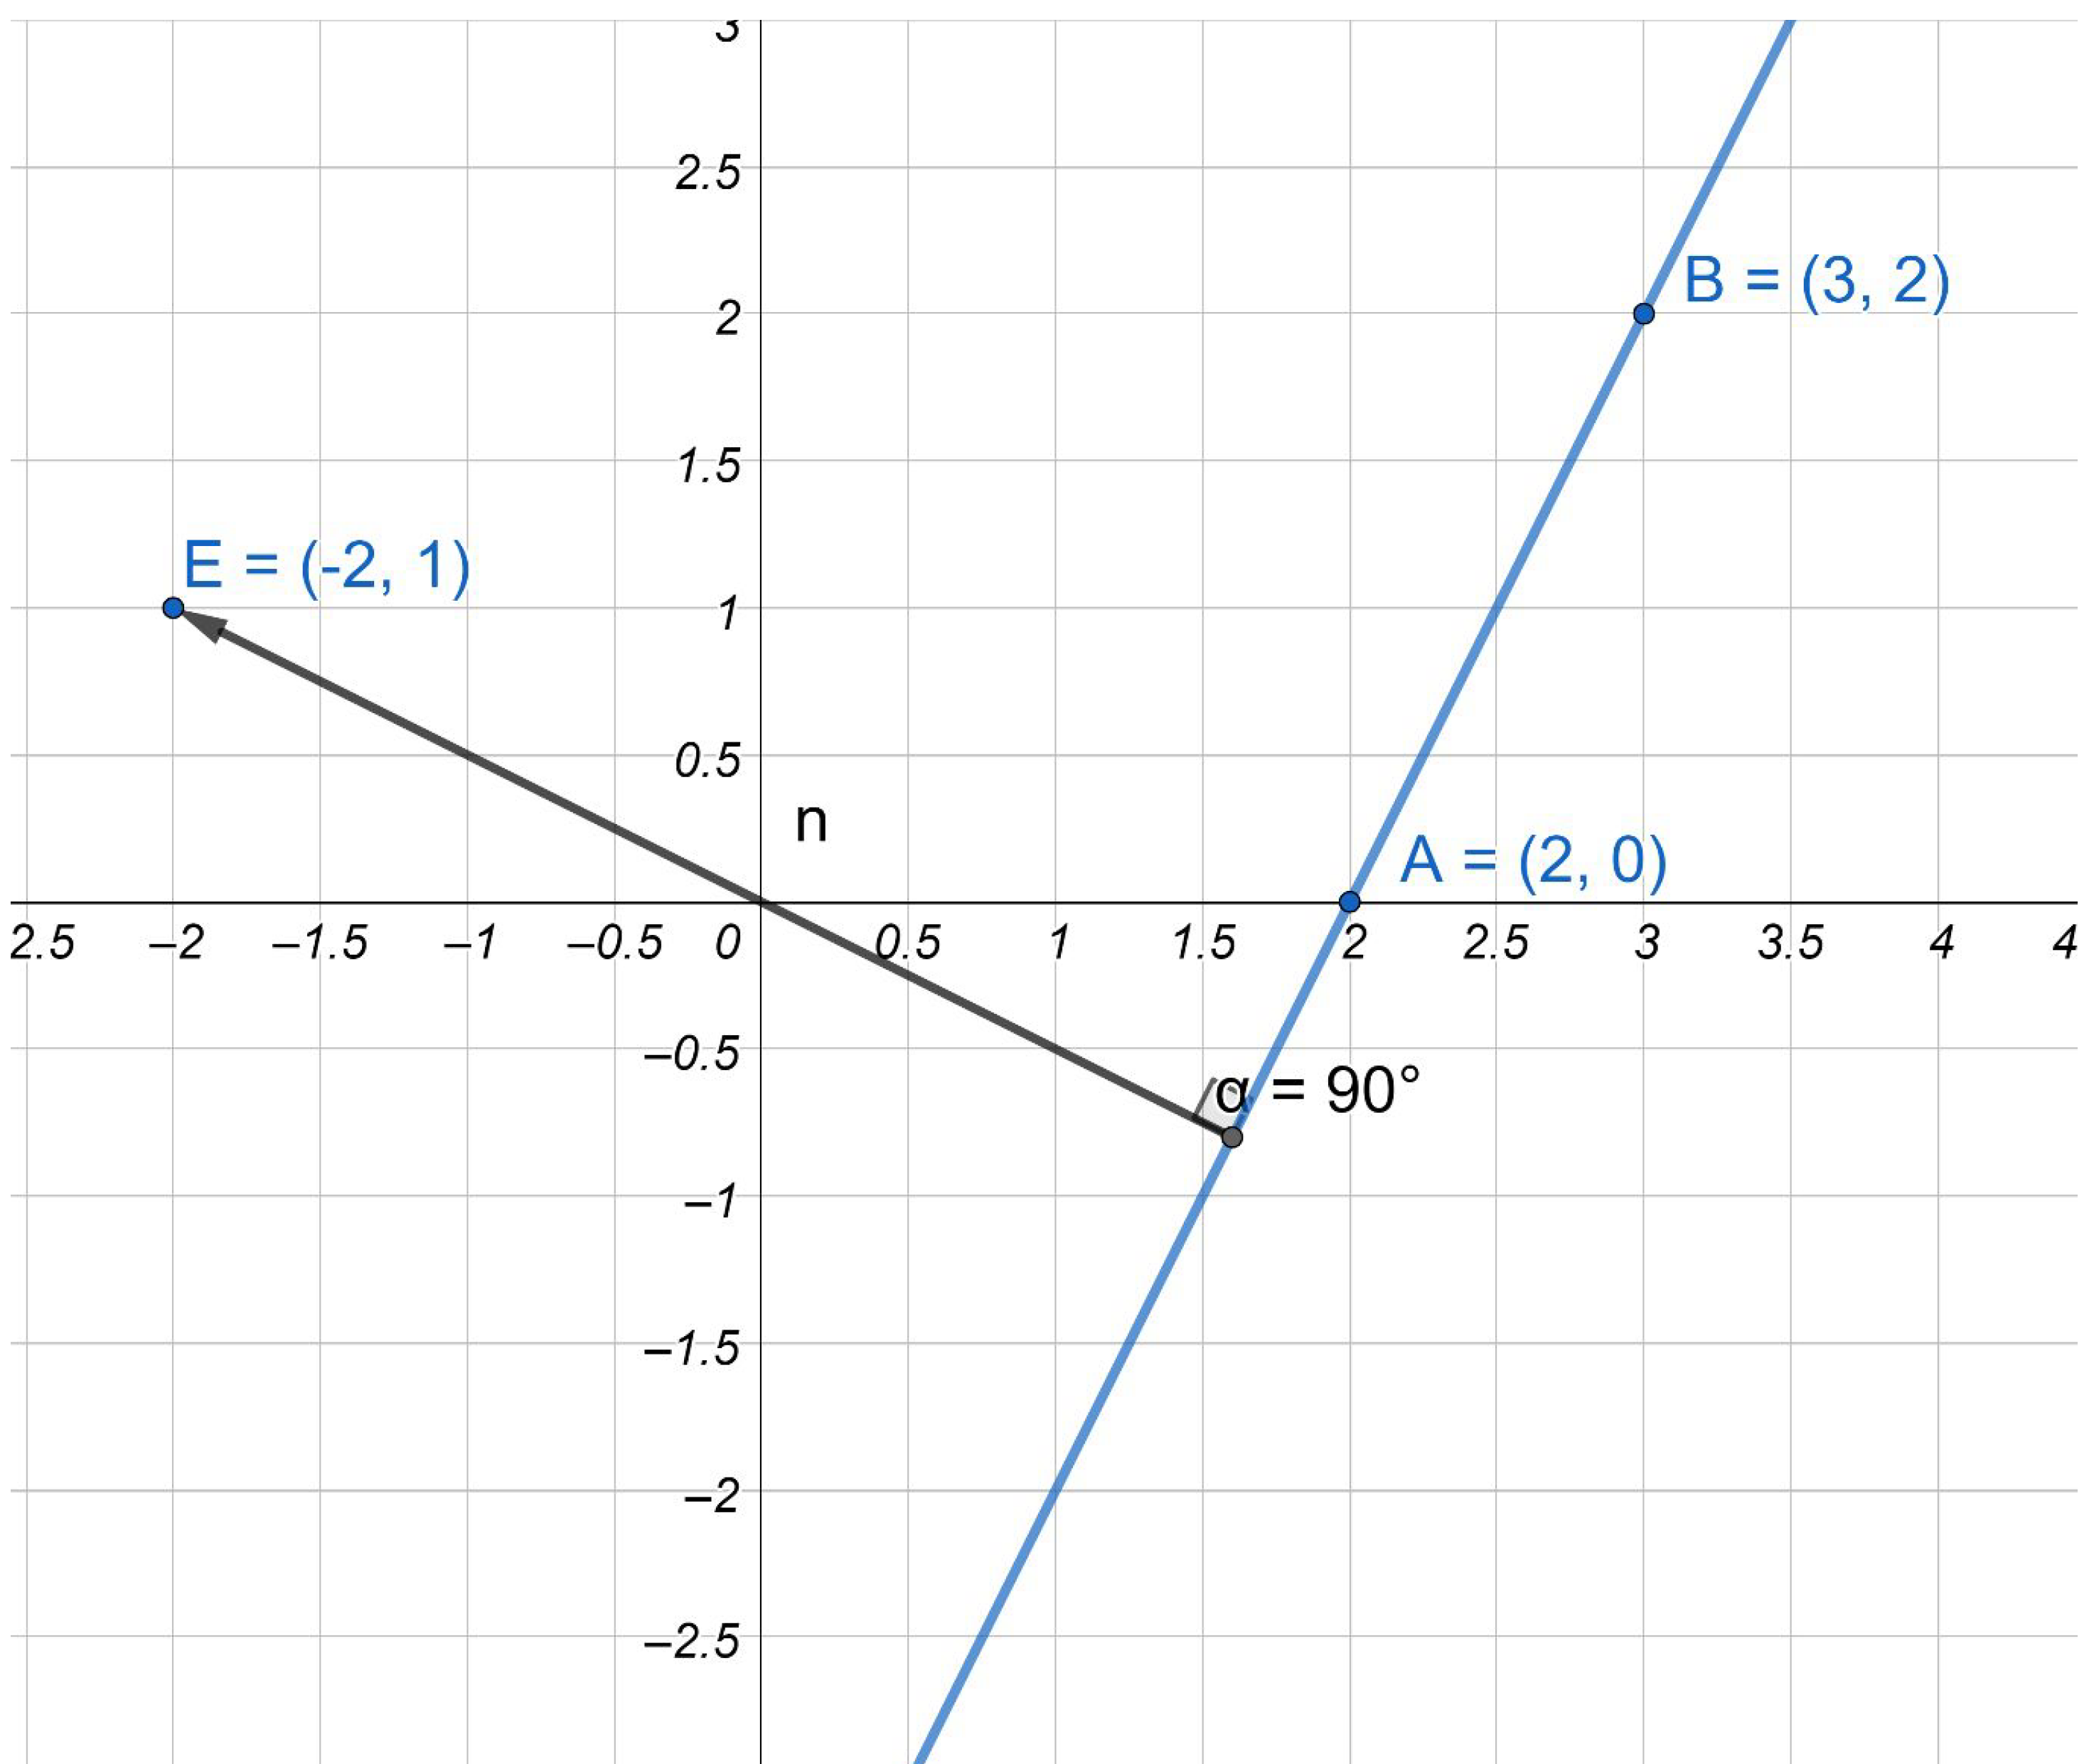
\includegraphics[height=6cm,width=1\textwidth,keepaspectratio]{line_in_plane_task.png}
            % \caption{caption_name}
            \label{fig:line_in_plane_task.png}
        \end{figure}
    \end{minipage}
\end{frame}

\begin{frame}[t]{Line in plane}
\framesubtitle{Task 0, Answer}
    \vspace{-0.6cm}
    \begin{figure}[H]
        \centering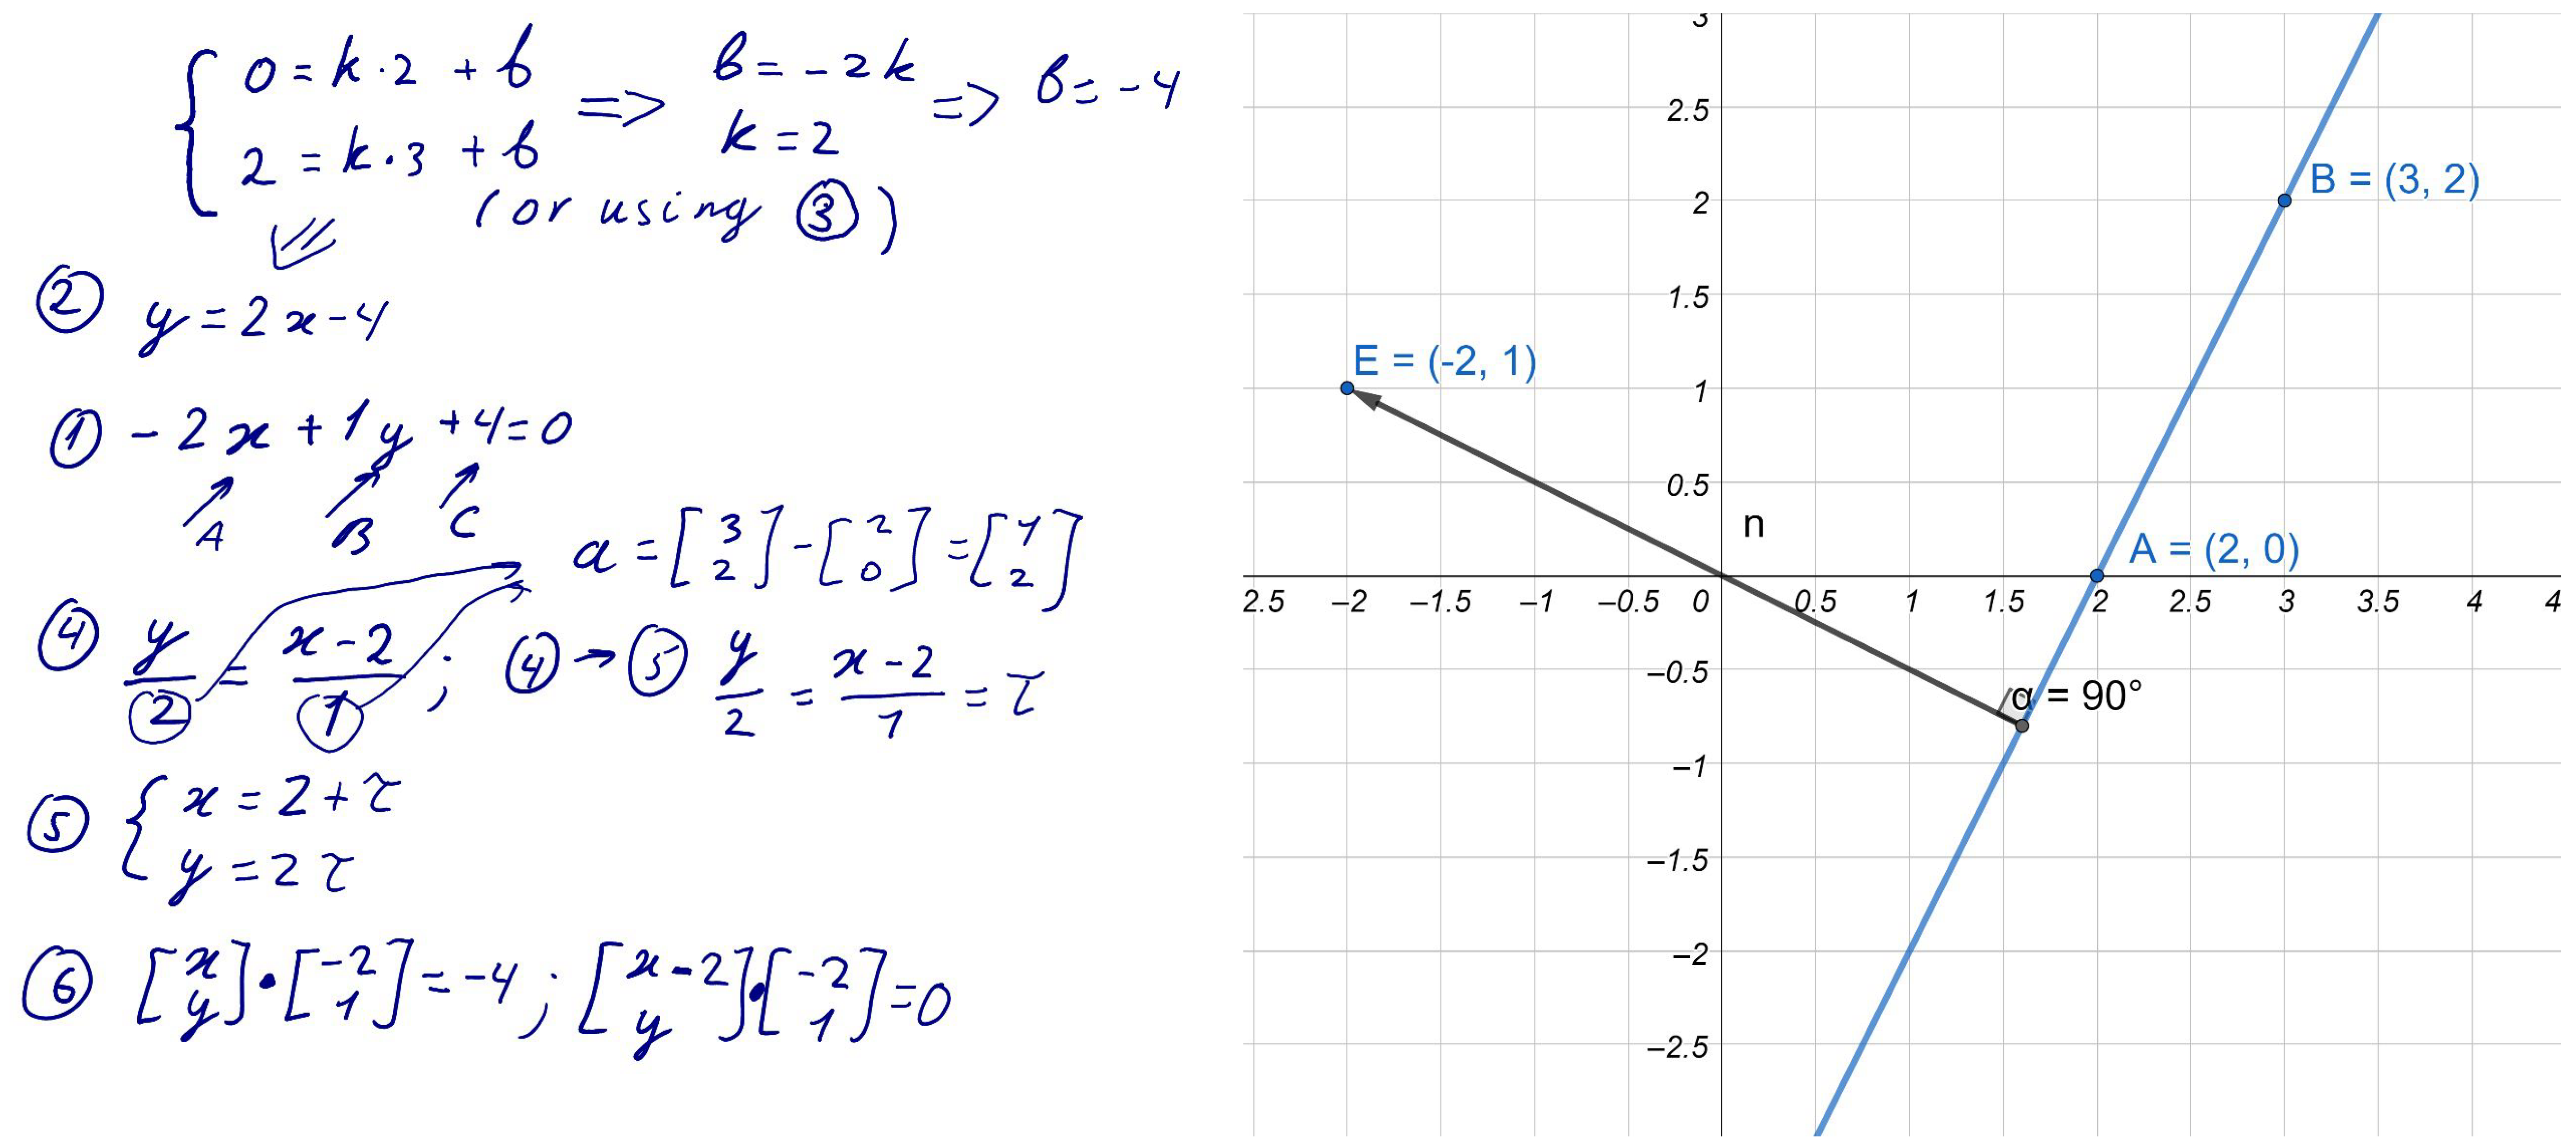
\includegraphics[height=6cm,width=1\textwidth,keepaspectratio]{line_in_plane_sol.png}
        \label{fig:line_in_plane_sol.png}
    \end{figure}
\end{frame}

\begin{frame}[t]{Task 1}
    \framesubtitle{}
    \only<1>{
        Find the slope of the line joining the points $(2, 3)$ and $(4, -5)$.}
    \only<2>{
        \alert{\Large Answer}
        \begin{figure}[H]
            \centering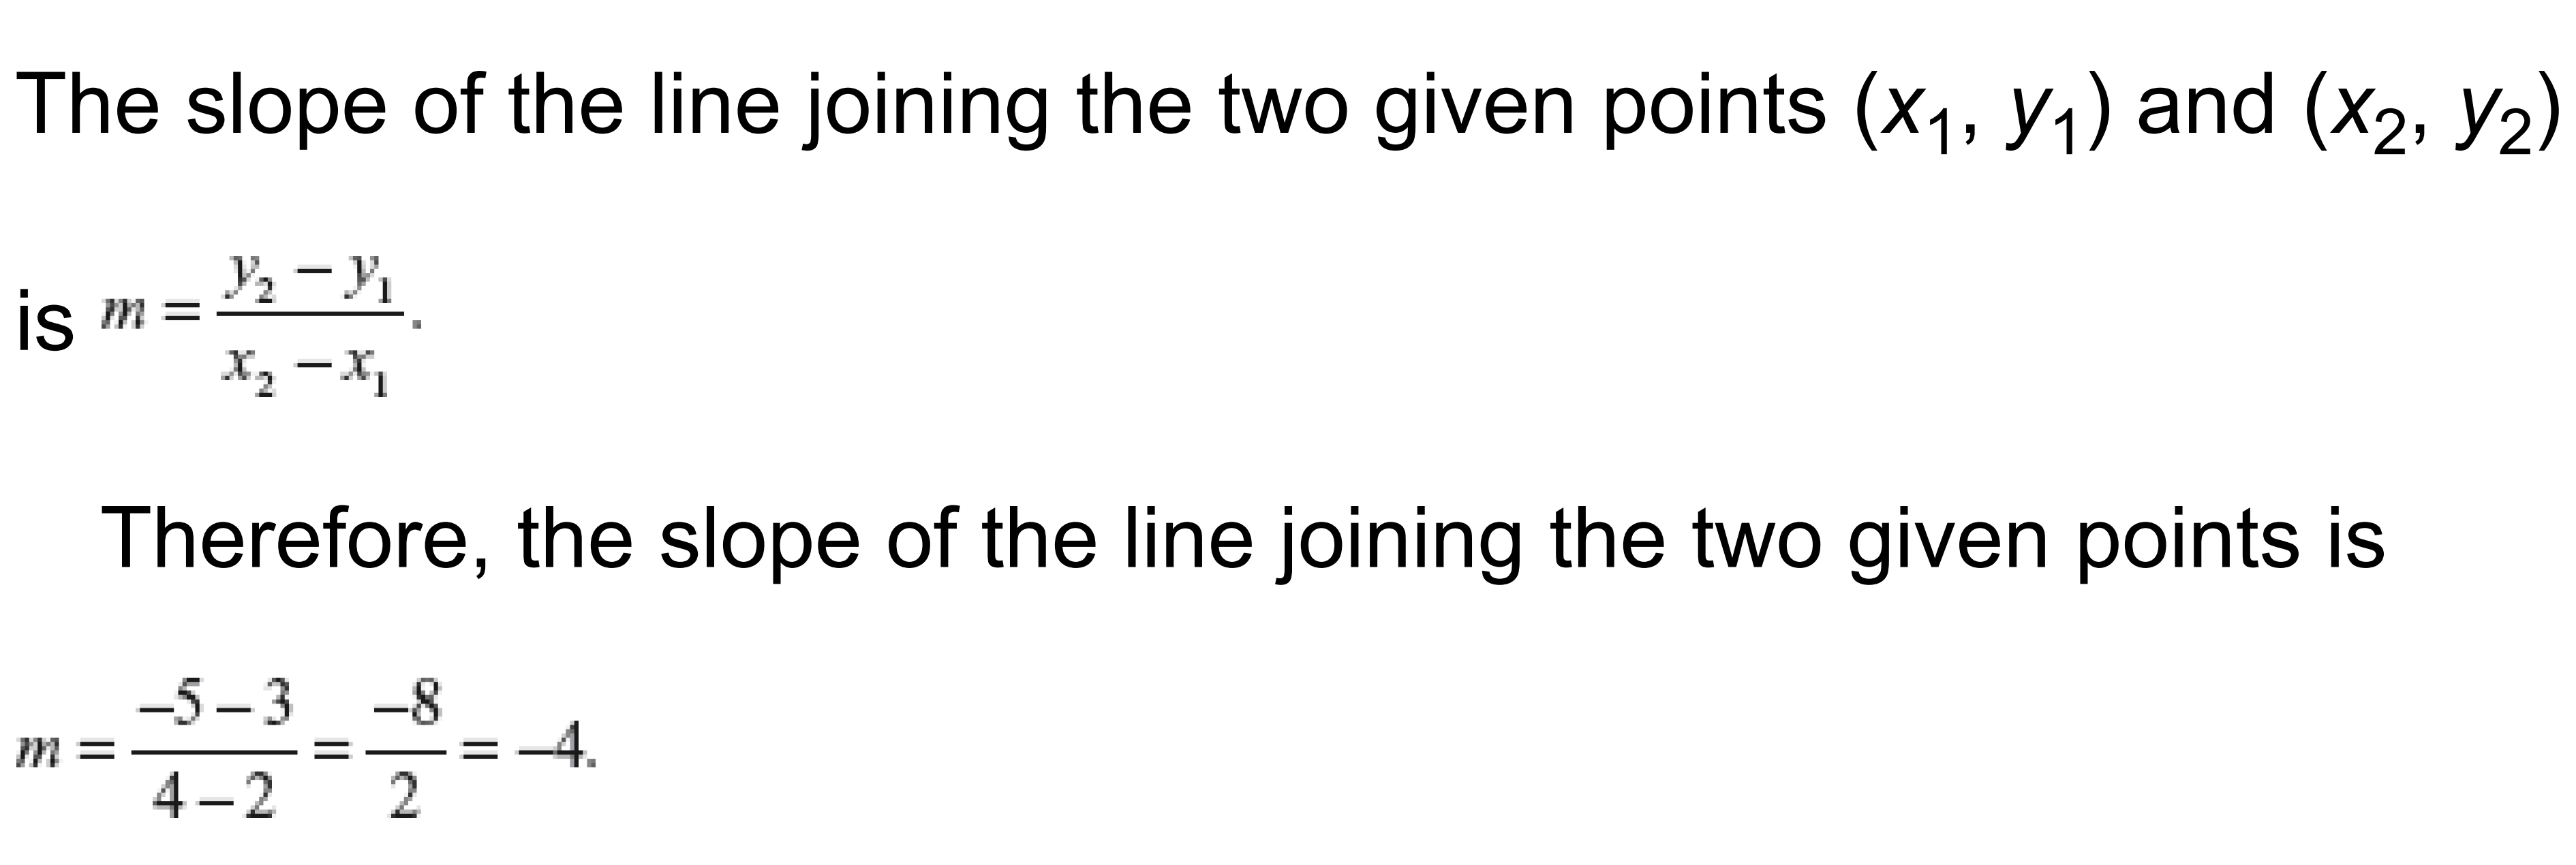
\includegraphics[height=5.5cm,width=1\textwidth,keepaspectratio]{1ans.png}
            % \caption{caption_name}
            \label{fig:1ans.png}
        \end{figure}
    }
\end{frame}

\begin{frame}[t]{Task 2}
    \framesubtitle{}
    \only<1>{
        Find the slope of the line $2x - 3y + 7 = 0.$}
    \only<2>{
        \alert{\Large Answer}
        \begin{figure}[H]
            \centering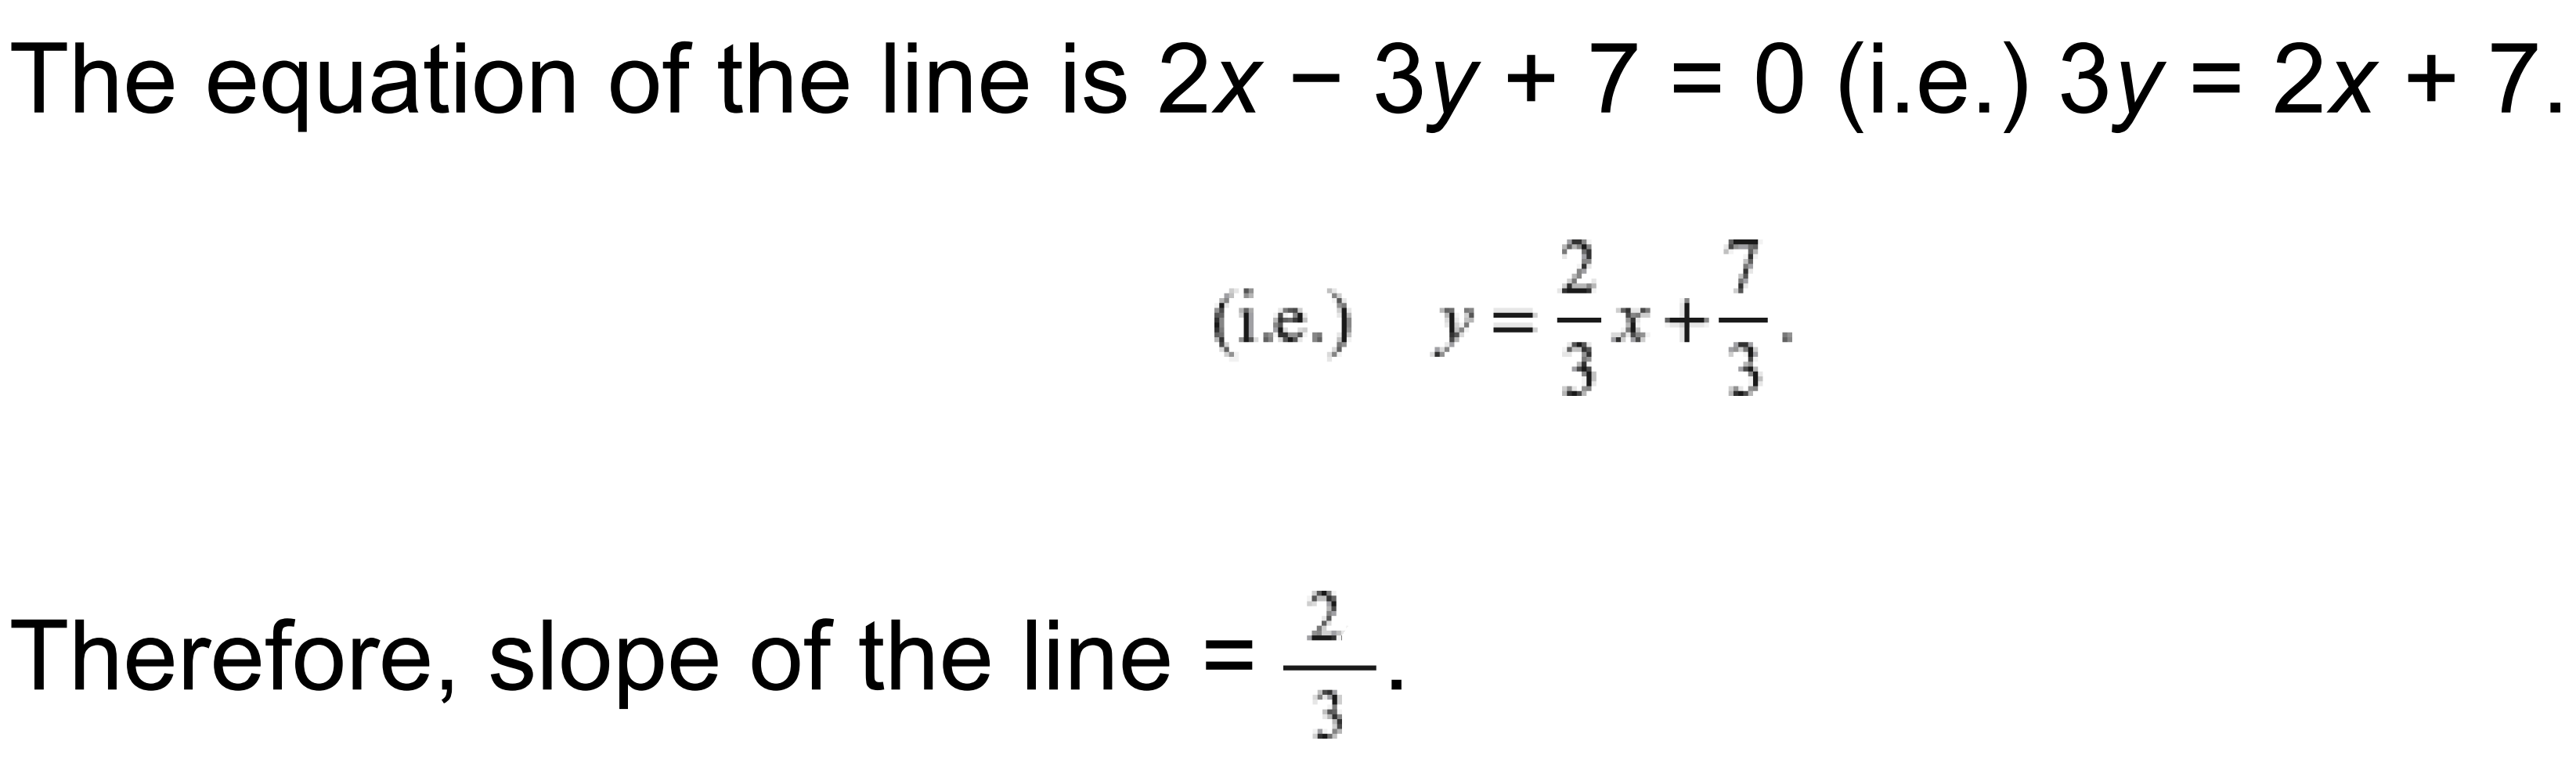
\includegraphics[height=5.5cm,width=1\textwidth,keepaspectratio]{2ans.png}
            % \caption{caption_name}
            \label{fig:2ans.png}
        \end{figure}
    }
\end{frame}

\begin{frame}[t]{Task 3}
    \framesubtitle{}
    \only<1>{
        Find the equation of the straight line, the portion of which between the axes is bisected at the point $(2, -5)$.}
    \only<2>{
        \alert{\Large Answer}
        \begin{figure}[H]
            \centering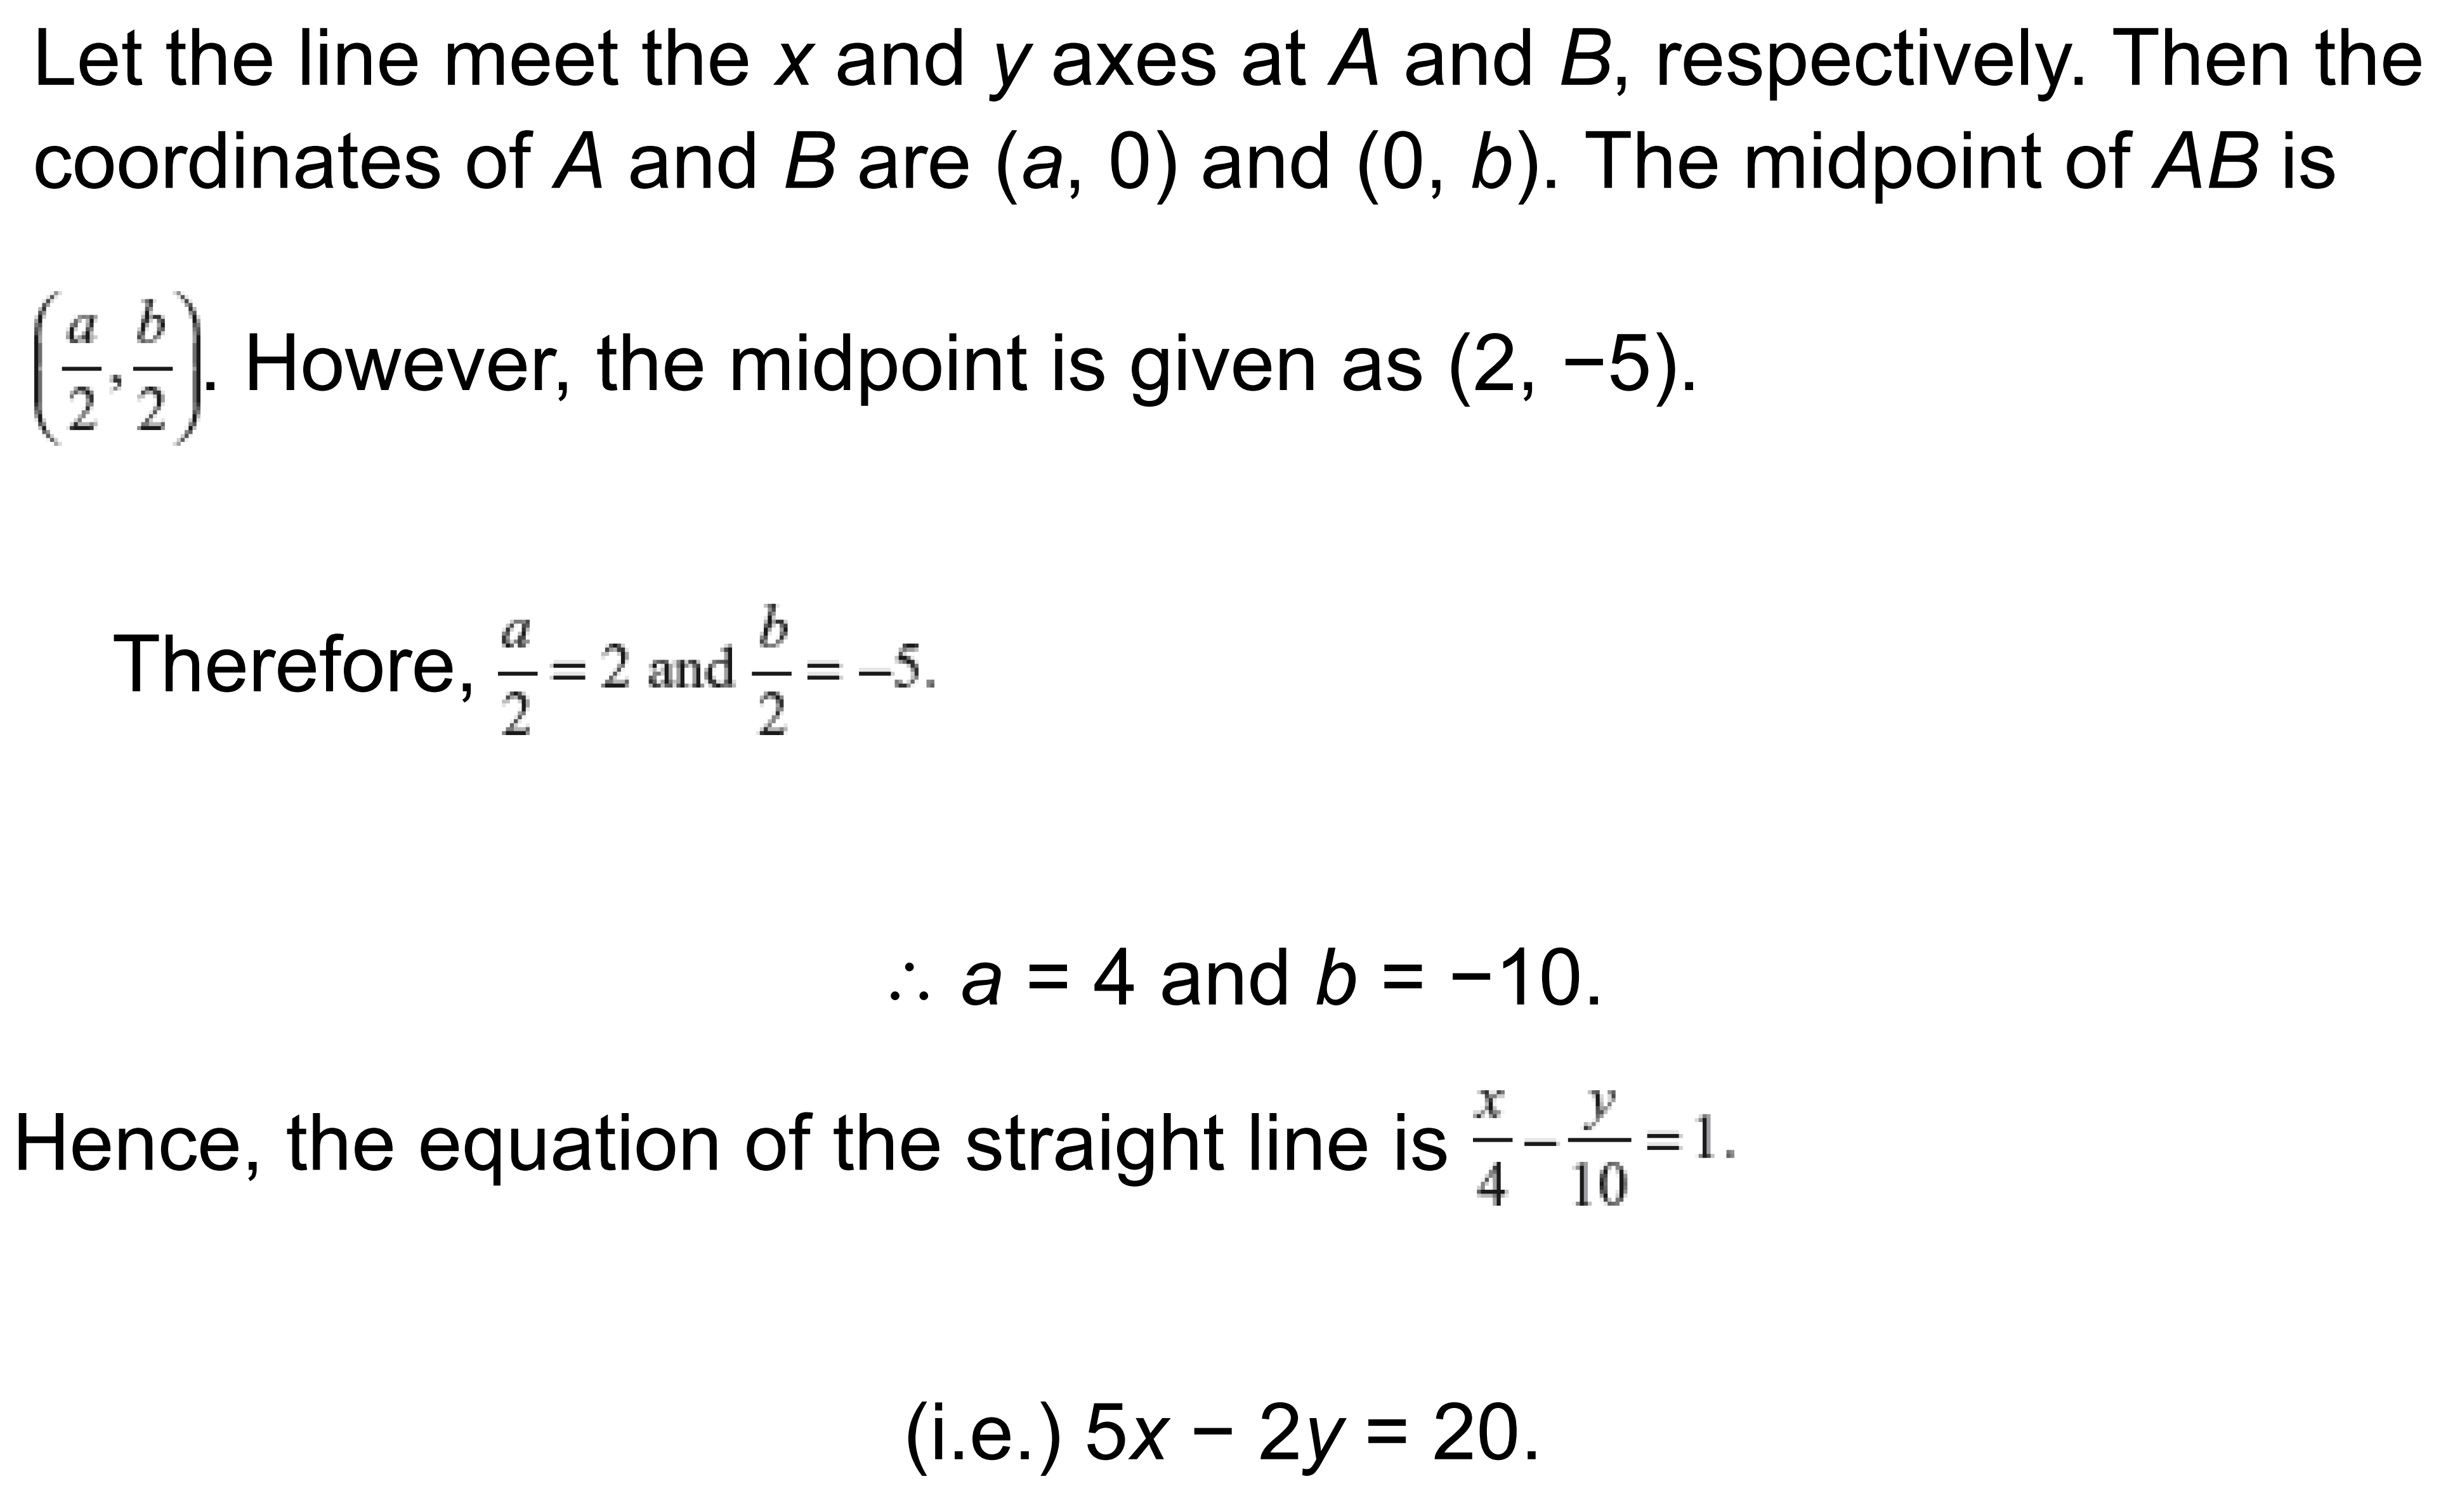
\includegraphics[height=5.5cm,width=1\textwidth,keepaspectratio]{3ans.png}
            % \caption{caption_name}
            \label{fig:3ans.png}
        \end{figure}
    }
\end{frame}

\begin{frame}[t]{Task 4}
    \framesubtitle{}
    \only<1>{
        \begin{minipage}{0.6\textwidth}
            Find the equation of the straight line concurrent\footnote{Lines are said to be cuncurrent if they are intersect at a single point} with the lines $2x + 3y = 3$ and $x + 2y = 2$ and also concurrent with the lines $3x - y = 1$ and $x + 5y = 11$.
        \end{minipage}
        \begin{minipage}{0.39\textwidth}
            \begin{figure}[H]
                \centering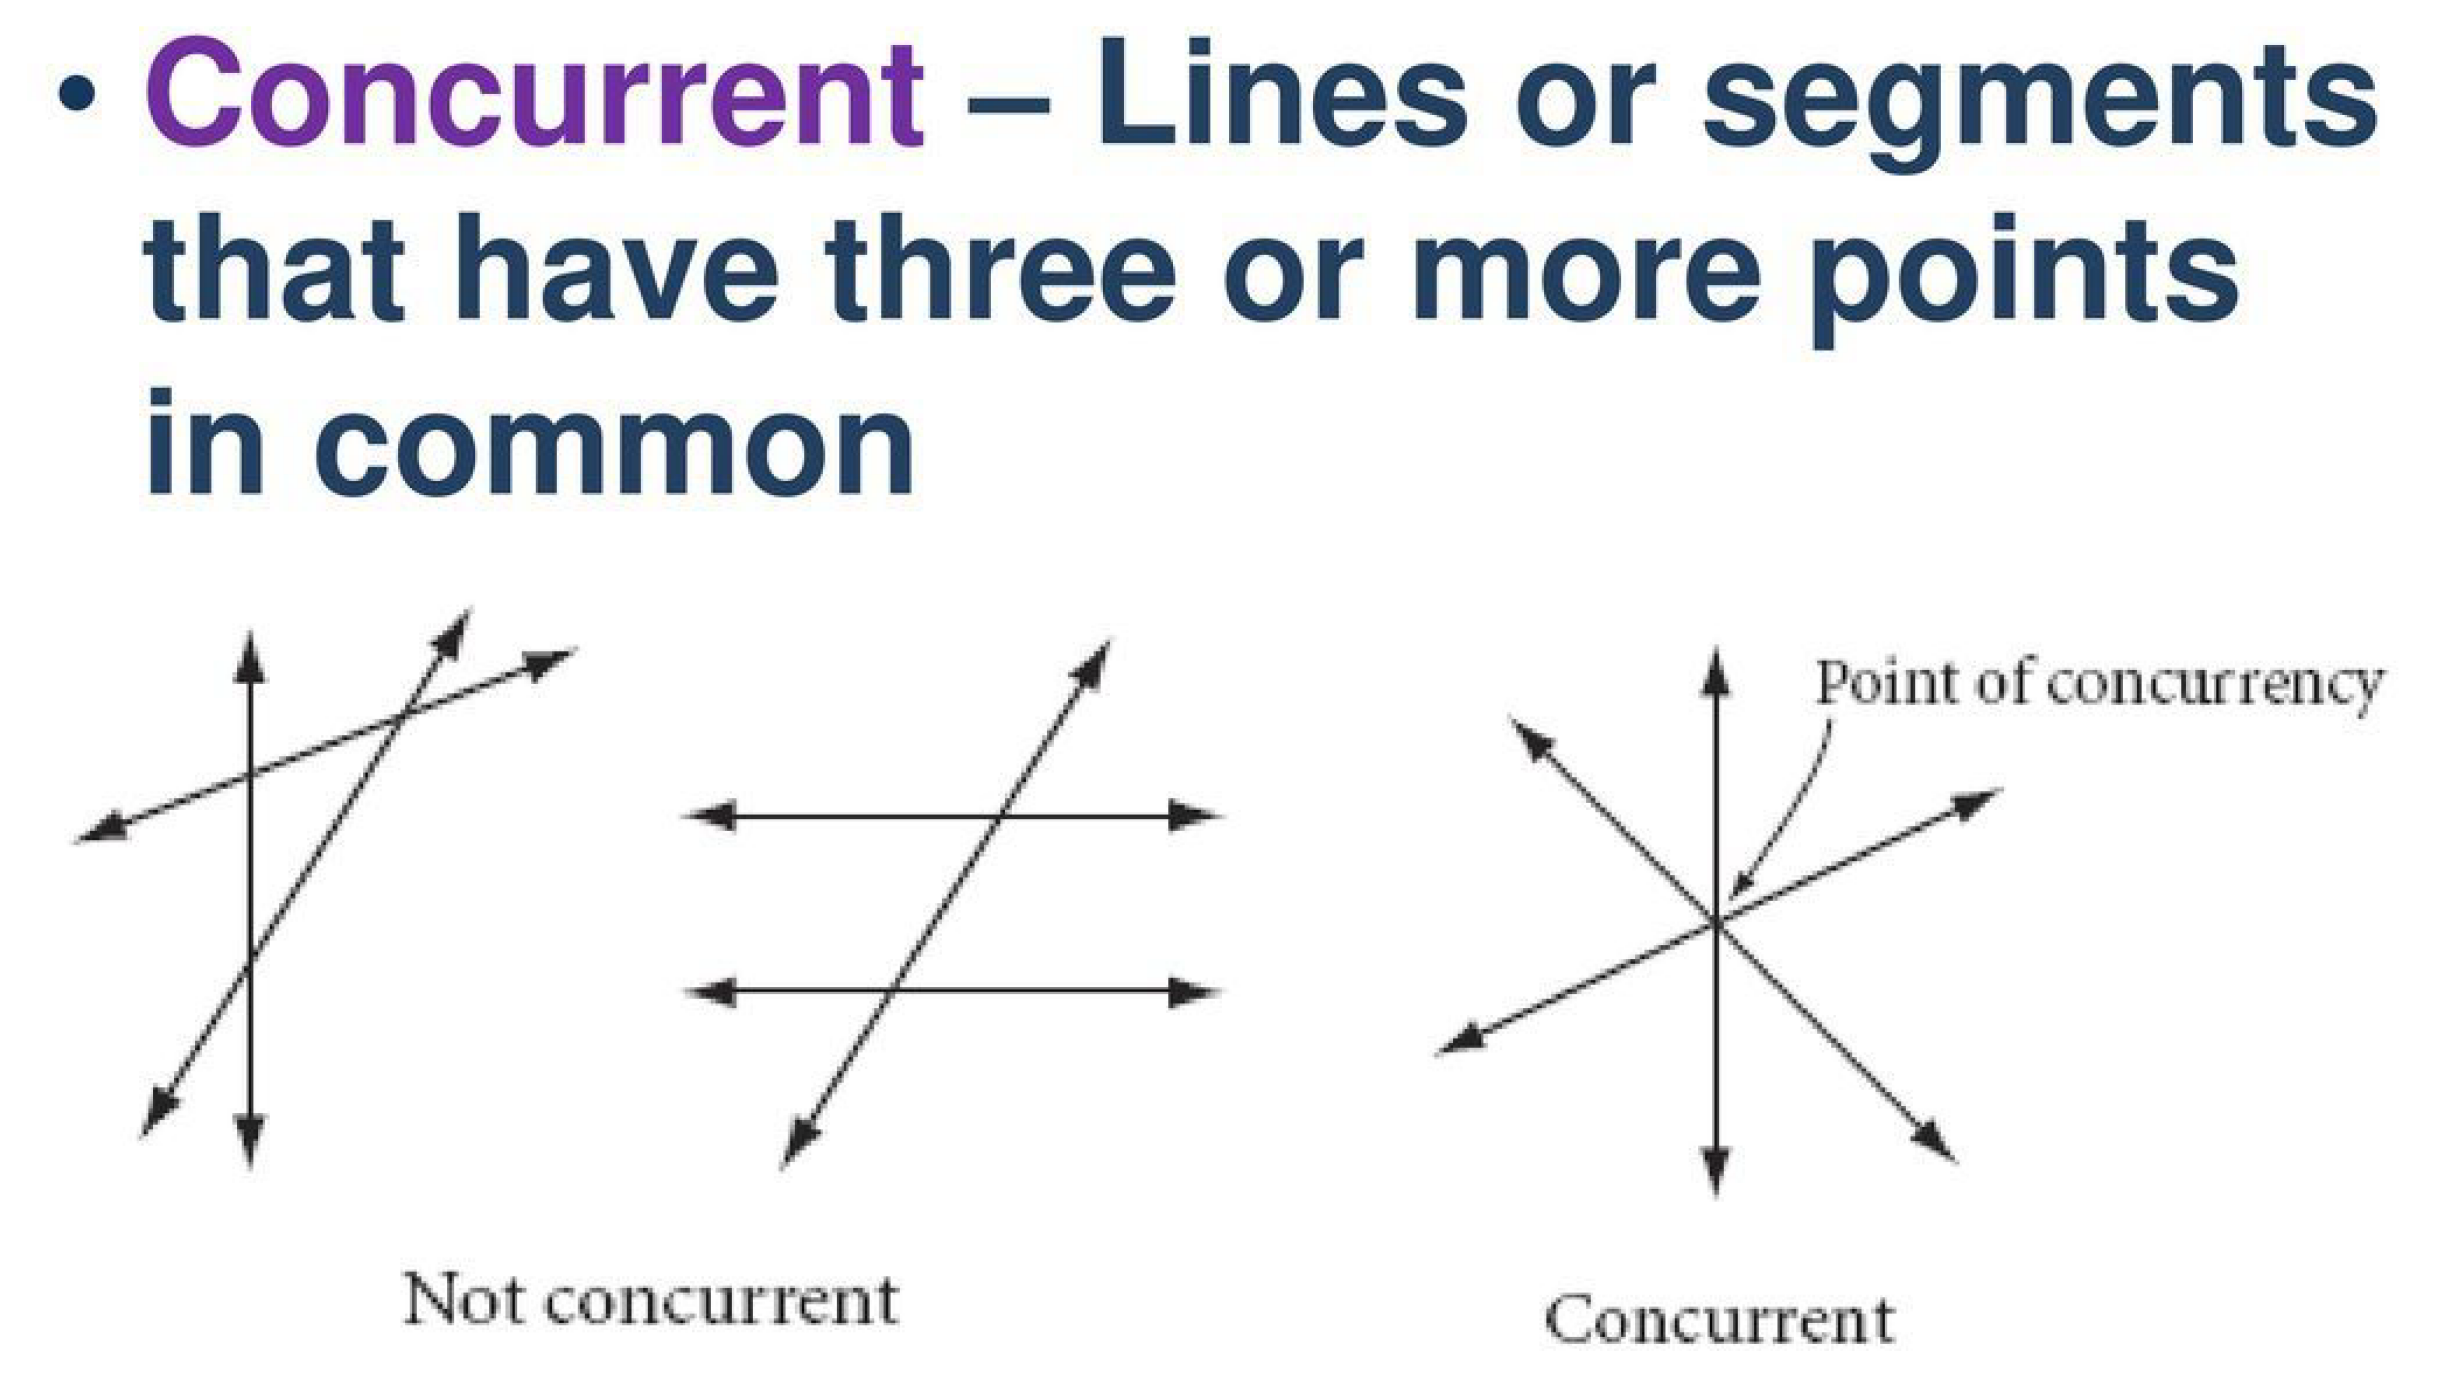
\includegraphics[height=6cm,width=1\textwidth,keepaspectratio]{concurrent_exp.png}
                % \caption{caption_name}
                \label{fig:concurrent_exp.png}
            \end{figure}
        \end{minipage}
        }
    \only<2>{
        \alert{\Large Answer}
        \begin{figure}[H]
            \centering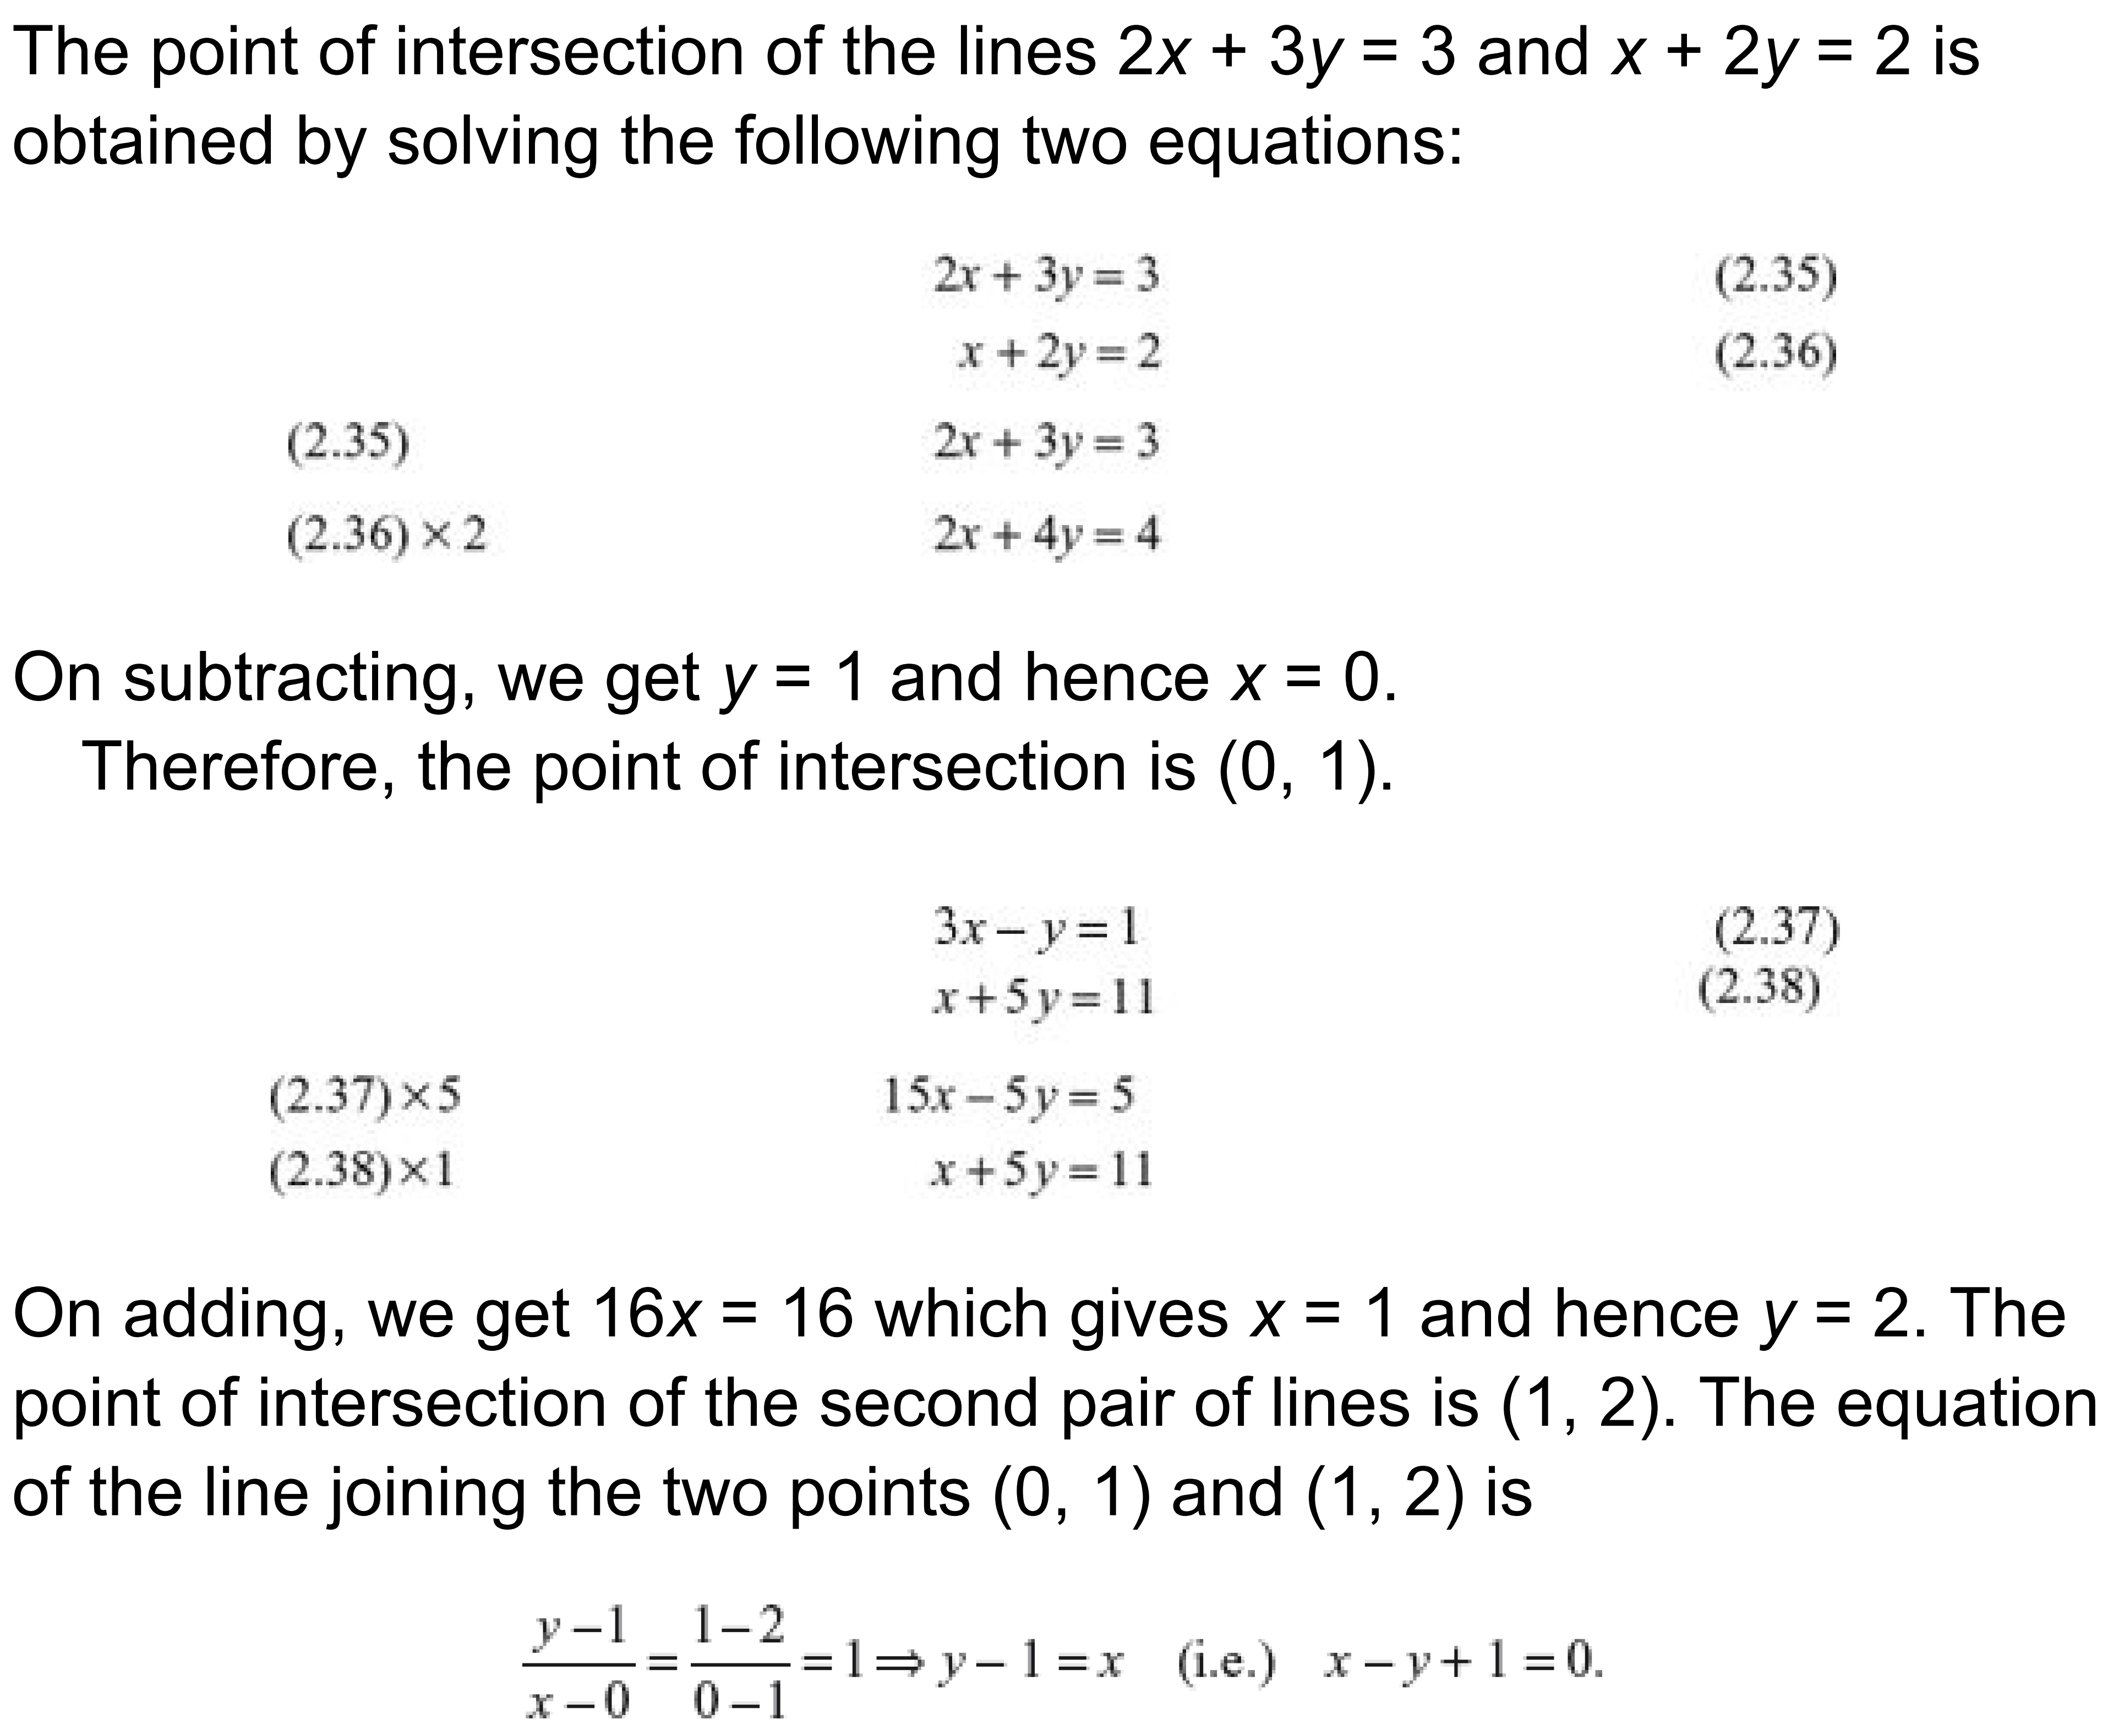
\includegraphics[height=5.5cm,width=1\textwidth,keepaspectratio]{4ans.png}
            % \caption{caption_name}
            \label{fig:4ans.png}
        \end{figure}
    }
\end{frame}

\begin{frame}[t]{Task 5}
    \framesubtitle{}
    \only<1>{
        $A(4, 1)$, $B(7, 4)$, and $C(5, -2)$ are the vertices of a triangle. Find the line equation which is goes from $A$ and perpendicular to $BC$.}
    \only<2>{
        \alert{\Large Answer}
        \begin{figure}[H]
            \centering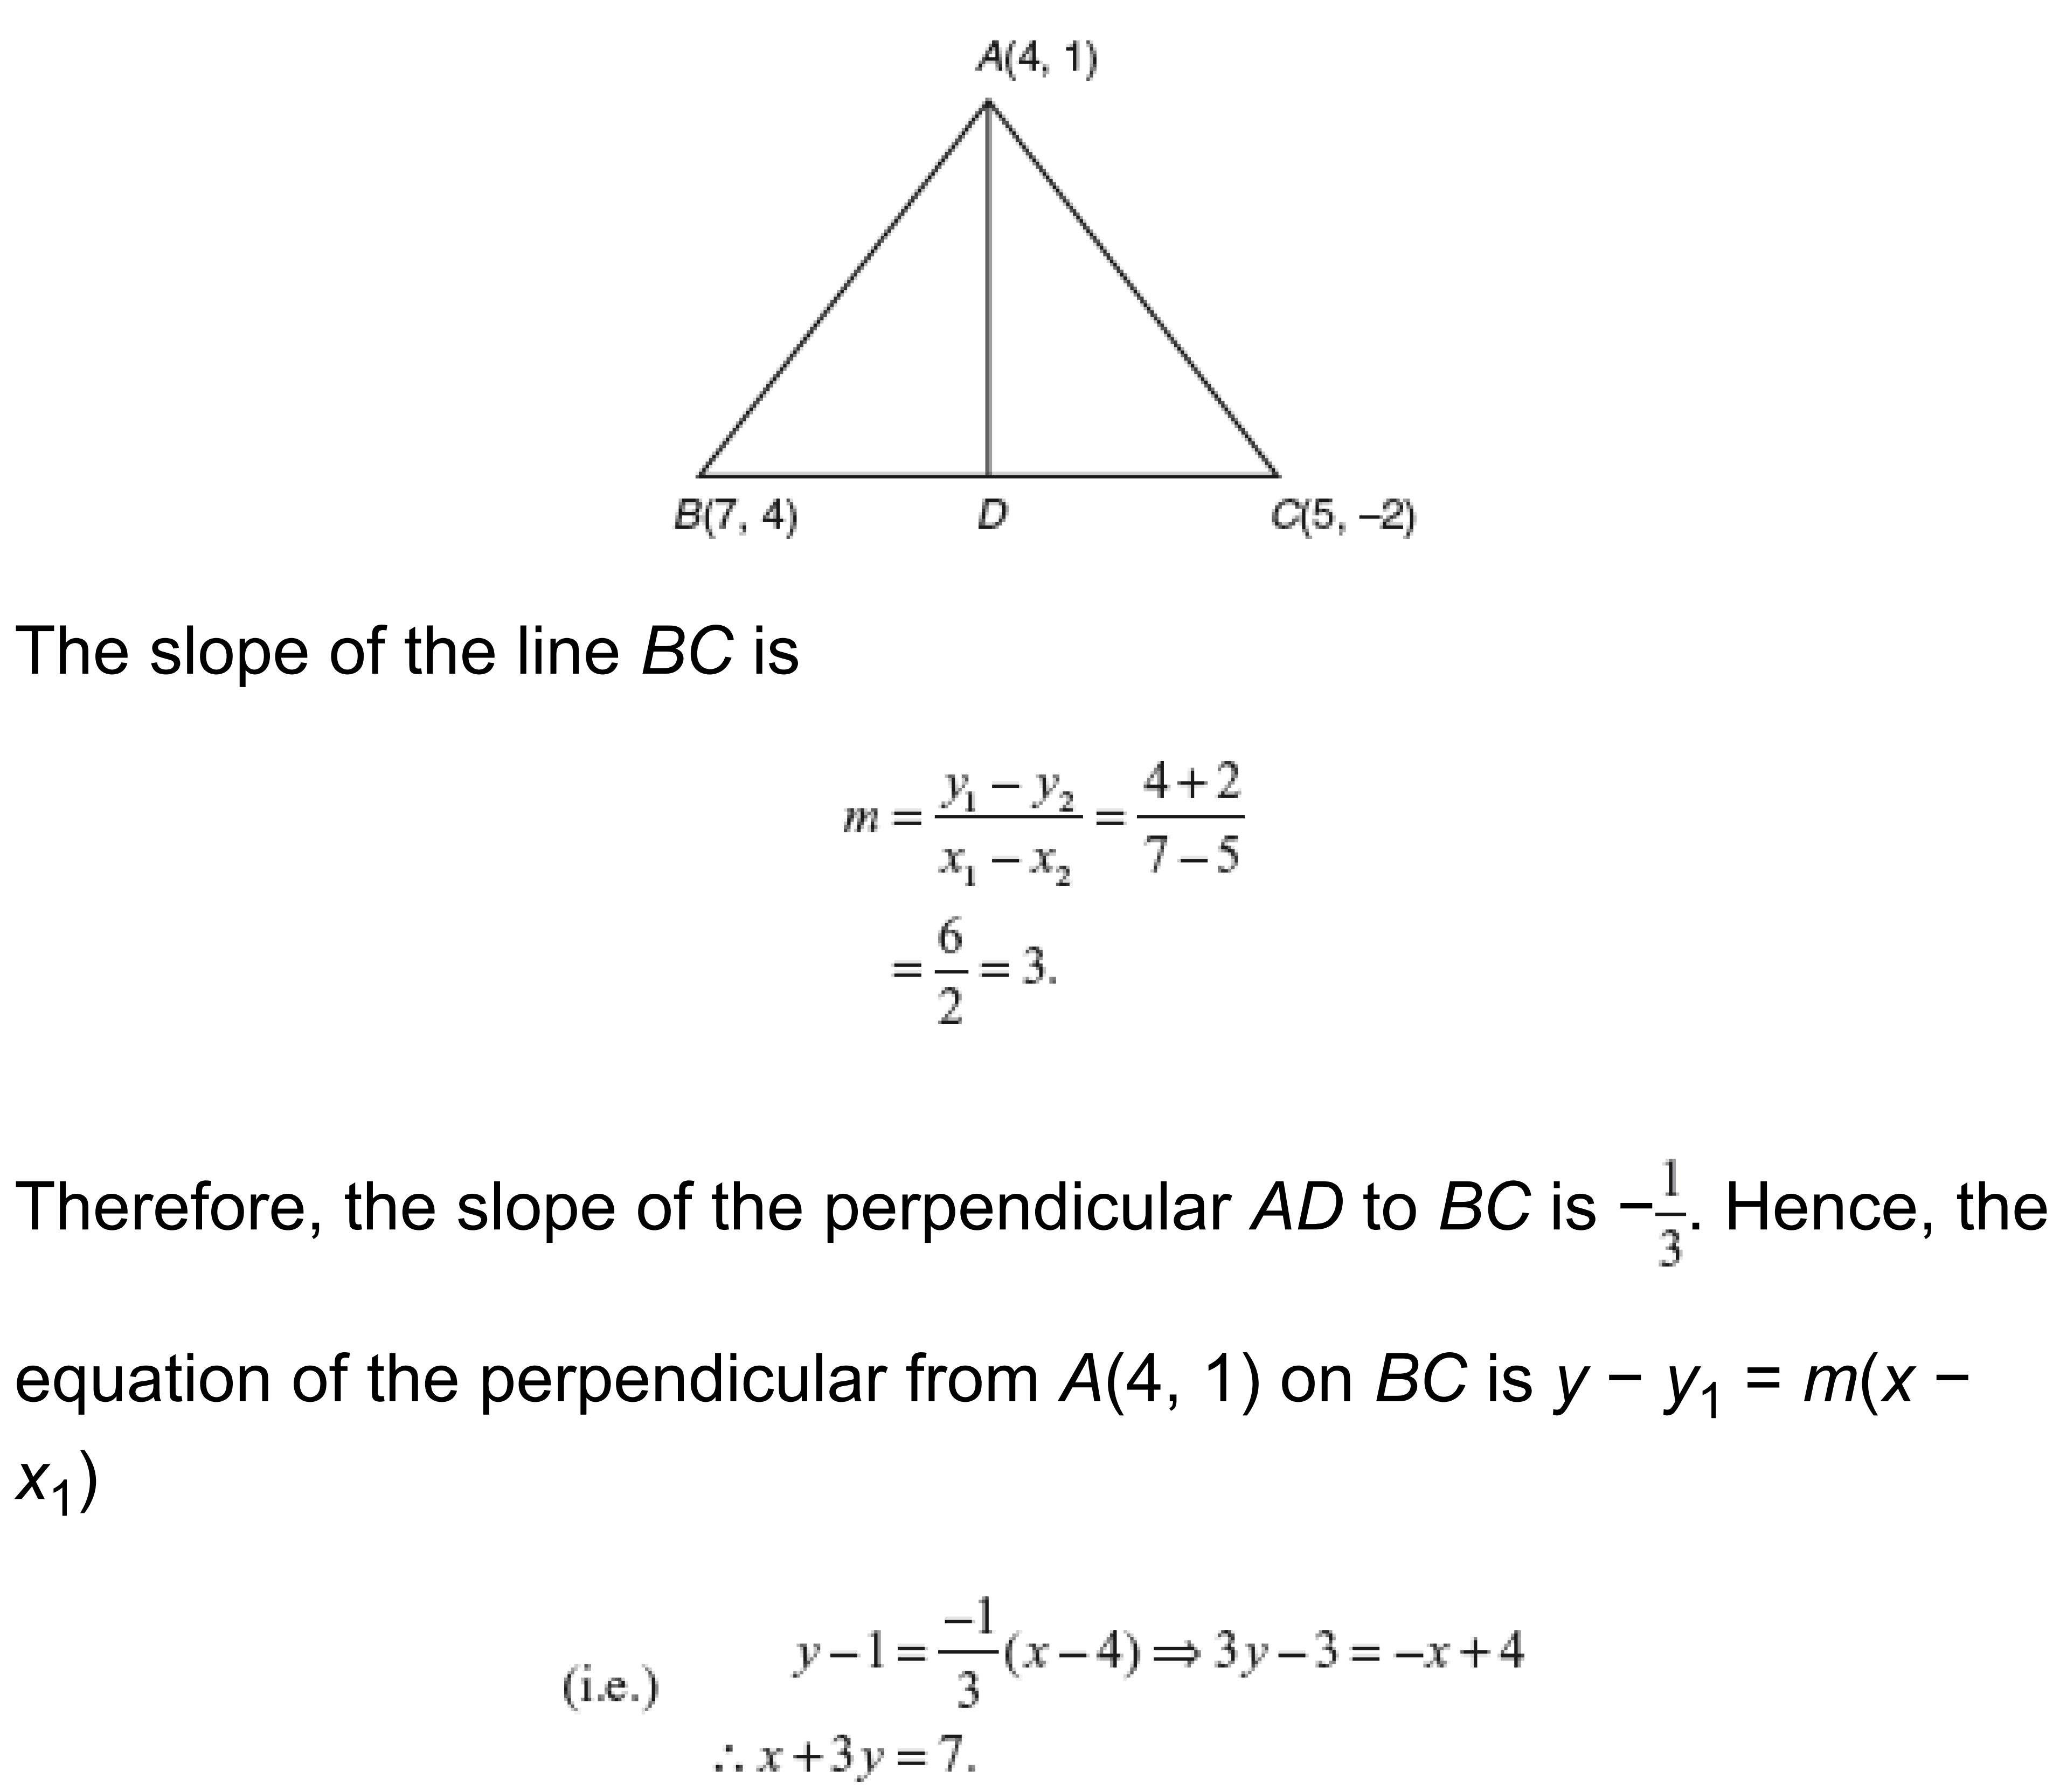
\includegraphics[height=5.5cm,width=1\textwidth,keepaspectratio]{5ans.png}
            % \caption{caption_name}
            \label{fig:5ans.png}
        \end{figure}
    }
\end{frame}

\begin{frame}[t]{Reference material}
    % \framesubtitle{OnlineMschool}
    \Large
    \begin{itemize}
        \item \href{https://en.wikipedia.org/wiki/Parametric_equation}{Parametric equation (Wiki)}
        \item \href{https://www.youtube.com/watch?v=3gbxDyivUx0}{Benefites of parametric form}
        \item \href{https://onlinemschool.com/math/library/analytic_geometry/line/}{Line in plane (OnlineMschool)}
    \end{itemize}
\end{frame}

\fbckg{fibeamer/figs/last_page.png}
\frame[plain]{}

\end{document}